% \documentclass{article}
% \usepackage[utf8]{inputenc}
% \begin{document}
% (Type your content here.)
% \end{document}

\documentclass[twoside]{article}

\usepackage[math]{kurier}
\usepackage[sc]{mathpazo}                   
\renewcommand{\sfdefault}{kurier}

\usepackage{fullpage,enumitem,amsmath,amssymb,graphicx}
\usepackage{float}
\newcommand{\R}{\mathbb{R}}
\usepackage{graphicx}
\graphicspath{ {imgs/} }


\usepackage{graphics}
\setlength{\oddsidemargin}{0.25 in}
\setlength{\evensidemargin}{-0.25 in}
\setlength{\topmargin}{-0.6 in}
\setlength{\textwidth}{6.5 in}
\setlength{\textheight}{8.5 in}
\setlength{\headsep}{0.75 in}
\setlength{\parindent}{0 in}
\setlength{\parskip}{0.1 in}


\newcounter{lecnum}
\renewcommand{\thepage}{\thelecnum-\arabic{page}}
\renewcommand{\thesection}{\thelecnum.\arabic{section}}
\renewcommand{\theequation}{\thelecnum.\arabic{equation}}
\renewcommand{\thefigure}{\thelecnum.\arabic{figure}}
\renewcommand{\thetable}{\thelecnum.\arabic{table}}


\newcommand{\lecture}[4]{
   \pagestyle{myheadings}
   \thispagestyle{plain}
   \newpage
   \setcounter{lecnum}{#1}
   \setcounter{page}{1}
   \noindent
   \begin{center}
   \framebox{
      \vbox{\vspace{2mm}
    \hbox to 6.28in { {\bf \sffamily AA 274: Principles of Robotic Autonomy
                        \hfill Winter 2018} }
       \vspace{4mm}
       \hbox to 6.28in { {\sffamily{\Large \hfill Lecture #1: #2  \hfill}} }
       \vspace{2mm}
       \hbox to 6.28in { {\it \hfill Scribes: #4} }
      \vspace{2mm}}
   }
   \end{center}
   \markboth{Lecture #1: #2}{Lecture #1: #2}

   \vspace*{4mm}
}



%%%%%%%%%%%%%%%%%%%%%%%%%%
%document
\begin{document}
%modify this
\lecture{4}{Robotic sensors and introduction to computer vision}{}{Qizhan Tam, Ben Goeing, Bilan Jackie Yang, Marc Deetjen}

\section{Introduction}

This lecture covers the performance characteristics of different types of sensors used in robots to detect their surroundings and introduces computer vision as used in robots. This paper will begin by first introducing the potential errors that can arise from using sensors, followed by characterizing the full spectrum of sensors. Lastly, we provide the basics of using computer vision to extract useful sensory information.

\section{Robotic Sensors}

\subsection{Motivation and Sensor basics}
To accomplish its objective, an autonomous system first requires knowledge about its environment. By using sensors to take measurements, the autonomous system will then be able to extract meaningful information from those measurements. For example, self-driving cars use multiple sensors such as laser range finders (LiDARs) usually mounted on the top, stereo cameras for visual recognition, GPS to track its global position, radar for long range detection and ultrasonic sensors for short range detection.
\subsubsection{Classification of Sensors}

\textbf{Proprioceptive}: Measures the internal robot parameters (e.g. motor speed, wheel load, robot arm joint angles, battery voltage etc.). \newline \newline
\textbf{Exteroceptive}: Acquires information from the robot's environment (e.g. distance measurements, light intensity, sound amplitude etc.). \newline \newline
\textbf{Passive}: Measures ambient environmental energy entering the sensor (e.g. temperature probes, microphones, CCD/CMOS cameras etc.). Challenge: environment has a significant influence on the sensor performance.\newline \newline
\textbf{Active}: Emits energy into the environment, then measure the environmental reaction (e.g. wheel quadrature encoders, ultrasonic sensors, laser rangefinders etc.). Challenge: emitted energy may affect environment and sensor may suffer interference from other signals. 


\subsubsection{Performance of Sensors}


The following design specs are often used to characterize the performance of sensors. They are basic Sensor Response /Performance Ratings that can be measured in laboratory environment.
\begin{itemize}
  \item \textbf{Dynamic Range}: The spread between the maximum and minimum input values to the sensor while maintaining normal sensor operation.
  \item \textbf{Resolution}: The minimum difference between two values that can be detected by a sensor.
  \item \textbf{Linearity}: The degree to which the sensor's output response depends linearly on the input.
 \item \textbf{Bandwidth/frequency}: The speed with which a sensor can provide readings (units of Hertz).
\end{itemize}

In Situ Sensor Performance 
The following performance metrics must be tested in a real environment:
\begin{itemize}
  \item \textbf{Sensitivity}: The degree to which a change in the target input changes the output signal.
  \item \textbf{Cross-sensitivity}: The sensitivity to environmental parameters that are unrelated to the target parameter (e.g. a navigational compass affected by nearby magnets).
  \item \textbf{Error (e)}: The difference between the sensor output \textit{m} and the true value, \textit{v}: $e:=m-v$
 \item \textbf{Accuracy (a)}: Conformity between the sensor's measurement and the true value: $a:=1-|e|/v$
 \item \textbf{Precision}: Reproductibility of the sensor results
\end{itemize}

\subsubsection{Uncertainty and Error propagation}
\textbf{Types of uncertainties and analysis strategy}
\begin{itemize}
    \item \textbf{Systematic errors}: Caused by factors that can in theory be modeled; they are deterministic (e.g. calibration errors).
    \item \textbf{Random errors}: Cannot be predicted with sophisticated models; they are stochastic (e.g. spurious range-finding errors).
    \item \textbf{Error analysis}: Performed via a probabilistic analysis. Common assumptions include a symmetric, unimodal, Gaussian distribution which is convenient, but often a coarse simplification. Error propagation is characterized by the error propagation law
\end{itemize}

\textbf{Challenges in characterizing error}
\begin{itemize}
    \item \textbf{Blurring of systematic and random errors}: Active ranging sensors have failure modes caused by certain relative positions of the sensor with environment targets (e.g. specular reflections from sonar sensors at specific angles to a smooth sheetrock wall).
    \item \textbf{Multimodal error distributions}: Behavior of a sensor's random error in terms of a probability distribution over various output values. One frequently assumes errors' probability distribution to have symmetry and unimodal distribution (e.g. sonar induces random error based on noise which exhibit symmetric and unimodal error characteristics).
\end{itemize}

\textbf{Representing Uncertainty}
\begin{itemize}
    \item \textbf{Statistical Representation}:
    With the true value being represented by X, the estimate of the true value  $E[X]$ given $n$ measurements with values $\rho_i$ is: $E[X]=g(\rho_1,\rho_2,...,\rho_n)$.
    The probability density function $f(x)$ is used to characterize the statistical properties of $X$. The sum of all probabilities is: $\int_{-\infty}^{\infty}f(x)dx=1$.
    The expected value $E[x]$ is represented by the mean: $\mu=E[X]=\int_{-\infty}^{\infty}xf(x)dx$ and the characterization of the range of possible values is defined as the variance: $Var(X)=\sigma^2=\int_{\infty}^{\infty}(x-\mu)^2f(x)dx$, where the standard deviation is $\sigma$.
    \item \textbf{Independence of random variables}:
    Frequently assumed in mobile robotics as a simplification, two random variables are independent if and only if: $E[X_1X_2]=E[X_1]E[X_2]$ and $Var(X_1+X_2)=Var(X_1)+Var(X_2)$
    \item \textbf{Gaussian Distribution/Normal Distribution}:
    The distribution is usually used for a random variable for which no better error model has been found. It is symmetric about mean $\mu$ and is unimodal with a peak at $\mu$. It has tails that approach zero asymptotically, which means that all errors are possible, but large errors may be highly improbable. The Gaussian probability density function only depends on the $\mu$ and $\sigma$: $f(x)=\frac{1}{\sigma\sqrt{2\pi}}exp\left(-\frac{\left(x-\mu\right)^2}{\sigma^2}\right)$
    
\end{itemize}
\subsection{Encoders}
Encoders are proprioceptive sensors that can be used for tasks such as robot localization. In mobile robotics, optical encoders are used to measure angular speed and position and to control the position or speed of wheels and other motor-driven joints. This is best done in the reference frame of the robot.

Encoders are electro-mechanical devices that convert motion into a sequence of digital pulses. They consist of an illumination source, a fixed grating to mask the light, a rotor disc with a fine optical grid that rotates with the shaft, and fixed optical detectors. During the rotation of the motor, the amount of light that strikes the optical detectors varies based on the alignment of the fixed and moving gratings. This results in a sine wave, which is transformed into a discrete square wave using a given threshold to distinguish between "light" and "dark" states. The Resolution is then measured in cycles per revolution (CPR). Typical encoders have around 2000 CPR.

In mobile robotics, quadrature encoder are often used, in which case a second illumination and detector pair is added at a 90-degree angle. This results in twin twin square waves, which provide additional information. (See Figure \ref{fig:encoder}).

\begin{figure}[H]
\centering
        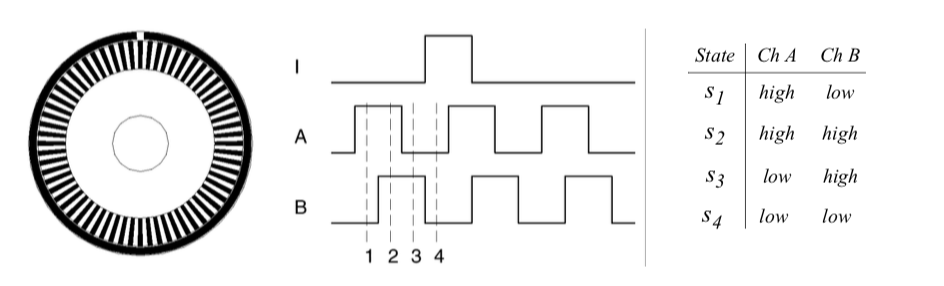
\includegraphics[width =11 cm]{Enc.png}
        \caption{Quadrature optical wheel encoder \cite{SNS}}
        \label{fig:encoder}
\end{figure}





\subsection{Heading sensors}
Heading sensors are used to determine the robot’s orientation and inclination. In combination with velocity information, they allow us to calculate a position estimate via integration. This process is referred to a dead reckoning.
\subsubsection{Compasses}
Compasses are an example of exteroceptive heading sensors. Digital compasses using the Hall effect are popular in mobile robotics. Using the earth's magnetic field, they provide a rough estimate of direction. They are inexpensive, but often suffer from poor resolution and accuracy. Flux gate compasses have improved resolution and accuracy, but come at a larger price and physical size. Both compass types are vulnerable to vibrations and disturbances in the magnetic field, and are therefore less well suited for indoor applications.

\subsubsection{Gyroscopes}
Gyroscopes are an example of proprioceptive heading sensors. They can provide an absolute measure for the heading of a mobile system. Mechanical gyroscopes contain an internal spinning wheel whose angular momentum keeps the axis of rotation inertially stable see Figure \ref{fig:gyro}. No torque $\tau$ can be transmitted from the outer frame onto the inner wheel, as it so proportional to the spinning speed $\omega$, the precision speend $\Omega$ and the wheel's inertia $I$, as represented by the formula $\tau = I\omega\Omega$. High quality gyroscopes still have an angular drift of about 0.1 per 6h, due to friction.

Optical gyroscopes are a relatively new invention. They use angular speed sensors with two monochromatic light beams, or lasers, emitted from the same source. Two beams are sent clock - and counterclockwise through an optical fiber. Since the laser traveling in the direction of rotation has a slightly shorter path, it will have a higher frequency. This frequency difference $\delta f$ is proportional to the angular velocity, which can therefore be estimated. In modern optical gyroscopes, bandwidth can easily exceed 100 kHz, while resolution can be smaller than 0.0001 degrees/hr



\begin{figure}[H]
\centering
        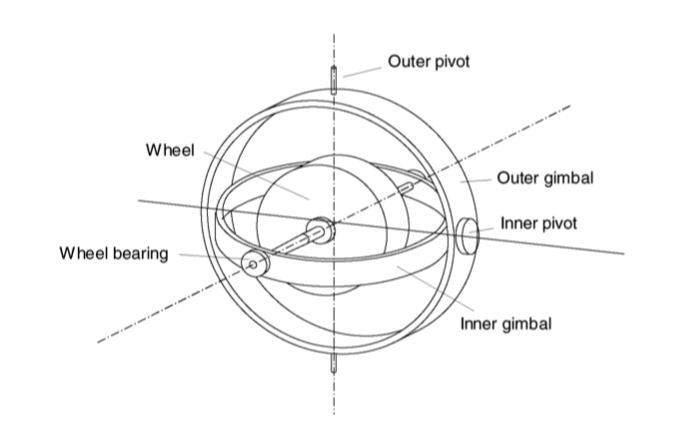
\includegraphics[width =8 cm]{gyro.png}
        \caption{Two-axis mechanical gyroscope \cite{SNS}}
        \label{fig:gyro}
\end{figure}





\subsection{Accelerometer}
An accelerometer is a device used to measure all external forces acting upon it, including gravity. Essentially it is a simple spring-mass-damper system that can be represented by this second order differential equation \cite{dudek2008inertial}:

$$F_{applied} = F_{inertial} + F_{damping} + F_{spring} = m \ddot{x} + c \dot{x} + k x$$

Where m is the proof mass, c is the damping coefficient, k is the spring constant, and x is the equilibrium case relative position. When a static force is applied, the system will oscillate until it reaches a steady state. Appropriate damping material and mass are chosen to ensure that the system can stabilize quickly and then the applied acceleration can be calculated as $a_{applied} = \frac{kx}{m}$ .

Modern accelerometers, like the ones in mobile phones, are usually very small, which is enabled by the Micro Electro-Mechanical Systems (MEMS) consisting of a cantilevered beam and a proof mass. The deflection of the proof mass from its neutral position is measured using the capacitive effect, which essentially measures the capacitance, or the piezoelectric effect, which measures an induced voltage. 

\begin{figure}[H]
  \centering
  \begin{minipage}[b]{0.15\textwidth}
    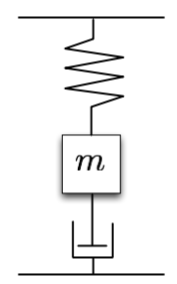
\includegraphics[width=\textwidth]{smd.png}
    \label{(a)}
  \end{minipage}
  \hfill
  \begin{minipage}[b]{0.7\textwidth}
    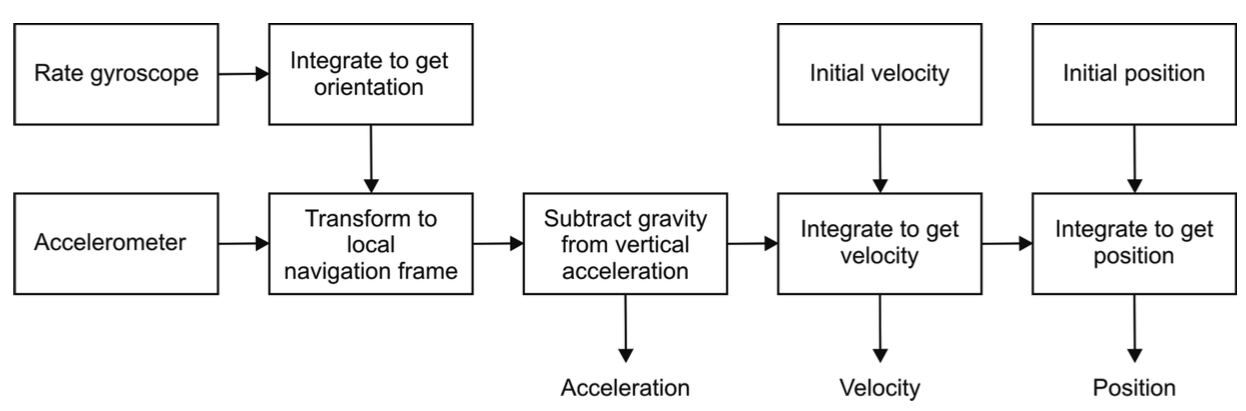
\includegraphics[width=\textwidth]{IMU.png}
    \label{(b)}
  \end{minipage}
\caption{(A) Working principle of the mechanical accelerometer; (B) IMU block diagram \cite{dudek2008inertial}}
\end{figure}

\subsection{Inertial measurement unit (IMU)}


% 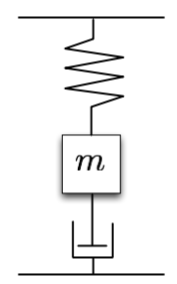
\includegraphics[scale=0.4]{smd.png}

An IMU is a device that uses gyroscopes and accelerometers to estimate the relative position, orientation, velocity, and acceleration of a moving vehicle with respect to an inertial frame. It integrates the information from gyroscopes to estimate the vehicle orientation and from accelerometers to obtain the instantaneous acceleration to understand the position of the vehicle based on initial conditions. A detailed working principle is shown in Figure \ref{fig:smd_IMU}. Through multiple times of integration, however, noises are accumulated over time, which result in the fundamental problem of drifting in IMUs. To cancel drift, periodic references to external measurements are required. Thus, IMUs are usually augmented with other techniques like GPSs or cameras to obtain some reference to absolute positions.

\subsection{Beacons}
Beacons are signaling devices with precisely known positions. An example from intuition is the lighthouse. Position can be determined by knowing the position of the beacon. More advanced examples of beacons are GPS, motion capture system for indoor use. With at least twenty-four operational GPS satellites at all times, the GPS synchronizes and reads data transmission from four satellites to obtain its own position based on the arrival time and instantaneous location. The four satellites provide three position axes plus a time correction. The localization resolution of GPS can be achieved using pseudorange with an extension method called differential GPS that uses a second receiver that is static at a known exact position to correct errors. 

\subsection{Active Ranging}

Active ranging sensors provide direct measurements of distance to objects in vicinity. These sensors are important for both localization and environment reconstruction. For example, they can be used for self-driving cars to know where the destinations are. There are two types of active ranging sensors. One is the time-of-flight active ranging sensors (e.g., ultrasonic, laser rangefinder, and time-of-flight camera) and the other is geometric active ranging sensors (optical triangulation and structured light).


\begin{figure} 
\centering
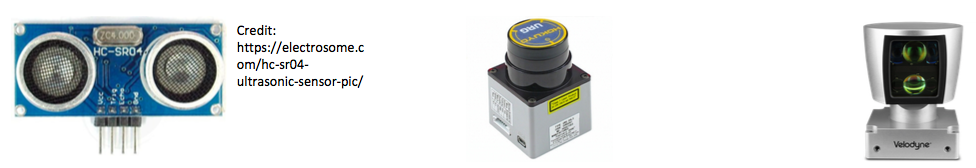
\includegraphics[scale=0.4]{ultra.png}
\caption{(A) Ultrasonic sensor; (B) laser rangefinder; (C) laser range sensor}
% \caption{This is a picture with scientific results.}\label{fig:grow}
\label{fig:active_range}
\end{figure}

\subsubsection{Time-of-flight Active Ranging}
Time-of-flight active ranging sensors make use of the propagation speed of sounds or an electromagnetic wave. The travel distance is given by 
$$d = c \cdot t$$
where d is the distance traveled, c is the speed of wave propagation, and t is the time of flight. Commonly used active ranging sensors are the ultrasonic sensor and LiDAR. Distance can be obtained by measuring the time form the transmission of the waves to detection of an echo. These waves could sound or light. Light sensors could be much more expensive because they are required to measure much shorter time but they also achieve much higher quality. LiDAR (Light Detection and Ranging) emits light beam and measure the time of return. Usually there are multiple emitters and receive multiple returns. LIDAR is often rotating to get 360 degree of view. The Performance depends on several factors, e.g., uncertainties in determining the exact time of arrival and interaction with the target.
\begin{figure} 
\centering
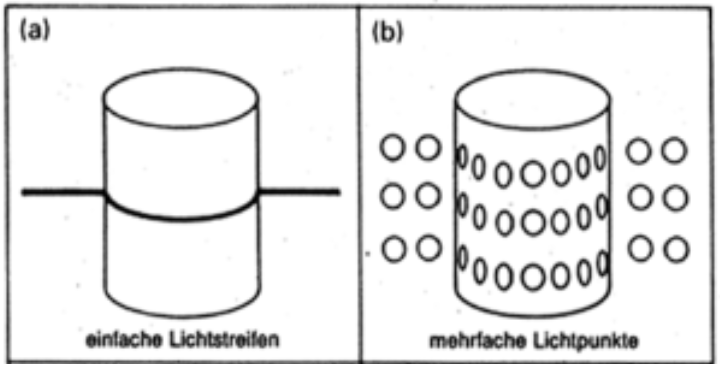
\includegraphics[scale=0.2]{light.png}
\caption{Possible light structures \cite{SNS}}
\label{fig:3D_light}
\end{figure}


\subsubsection{Geometric Active Ranging}
Geometric active ranging sensors use geometric properties in the measurements to establish distance readings. Optical triangulation sensors (1D) transmit a collimated beam toward the target and use lens to collect reflected light and project it onto a position-sensitive device or linear camera. Structured light sensors (2D or 3D) project a known light pattern (e.g., point, line, or texture) onto the environment. The reflection is captured by a receiver and then, together with known geometric values, range is estimated via triangulation. Figure \ref{fig:3D_light} shows systems that project light textures. CCD or CMOS receiver can then take photos and filter these images to identify the pattern’s reflection based on the geometrical deformation of the pattern of light. 
\subsection{Other Sensors}

Some classical examples of other sensors include radars that use Doppler effect to produce velocity data. Tactile sensors are critical to mobile, autonomous robots and are well understood and easily implemented. Some emerging technologies include artificial skins for obtaining tactile measurements and neuromorphic camera that detect motions with neurons spiking in changes of illumination. For example, small drones are often equipped with neuromorphic cameras which has very small power consumption.


\section{Introduction to computer vision and cameras}
Whereas most sensors require contact or an active signal to interact with their environment, vision sensors simply capture light rays that are already emitted by the environment. Vision is thus a powerful sensing method that can be defined as: the ability to interpret the surrounding environment using light in the visible spectrum reflected by objects in the environment. The most familiar vision sensor, the human eye, is an incredible example of a vision sensor because it captures an enormous amount of information on the order of millions of bits of information per second.

\subsubsection{History of cameras}

While the human eye has existed for thousands of years, the ancient idea of cameras has only been developed extensively more recently. Specifically, while the basic idea of a camera has existed for thousands of years, the first clear description of one was given by Leonardo Da Vinci in 1502 and the oldest known published drawing of a camera obscura, a dark room with a pinhole to image a scene, was shown by Gemma Frisius in 1544. By 1685, Johann Zahn had designed the first portable camera, and in 1822, Joseph Nicephore Niepce took the first physical photograph. Photography was born.

A modern camera in general can be defined as a sensor that captures light, converts that signal into a digital image, after which that image can be processed to filter desired information. These cameras capture images digitally by converting light into electric charge and processing it into electronic signals by one of two primary methods. Charge-Coupled Device (CCD) sensors transport charges from light rays across the chip so that it can be read into a voltage and recorded, whereas Complementary Metal-Oxide Semiconductor (CMOS) sensors use a transistor in each pixel combined with more traditional wires to record each pixel individually. Because CMOS sensors can be fabricated using traditional processes similar to microprocessor production, they are usually much cheaper than CCD sensors. Another benefit is that CMOS sensors consume much less power. However, CCD sensors usually have higher quality in terms of noise reduction and higher light sensitivity. Deciding which to use is application dependent.

\subsubsection{Camera basics: the pinhole camera}

The basic idea of a camera, meaning a sensor that captures light, involves an understanding of light rays. Light rays first originate from a light source, which emits them in various wavelengths and directions. Averaged over time, the emitted wavelengths and directions can be precisely described using a probability distribution function specific to the characteristics of the light source. When the light rays strike an object, they either directly reflect, scatter, or are absorbed depending on the surface properties of the object and the wavelength of the light. For example, an object looks blue because blue wavelengths of light are primarily scattered off the surface while other wavelengths are absorbed, a black object looks black because it absorbs most of the light rays, and a perfect mirror reflects all visible wavelengths of light.

Cameras work by capturing these light rays on some sort of photoreceptive surface in an organized way. As we see in Figure \ref{fig:LightRays}A, if we simply place a planar photoreceptive surface, or image plane, in front of an object, light rays that scattered from multiple different locations on the object will arrive at similar locations on the image plane and only an extremely blurred image of the object will be recorded. A solution to this blurring issue, as seen in Figure \ref{fig:LightRays}B, is to add a barrier that blocks off most of the light and only lets light through an aperture, or pinhole. Based on the geometry of this new system, if a light ray is absorbed in a certain location on the image plane, we know where that light ray last bounced off of an object. Namely, the light ray must have scattered from an object somewhere along the vector extending into space that connects the detected position on the image plane and the pinhole. In other words, the image plane will capture a picture of the object and surrounding scene because the geometry of the camera constrains the light rays that are captured. However, as captured by the photograph, the size of object is ambiguous and can only be determined if one knows how far away the object lies.

\begin{figure} 
\centering
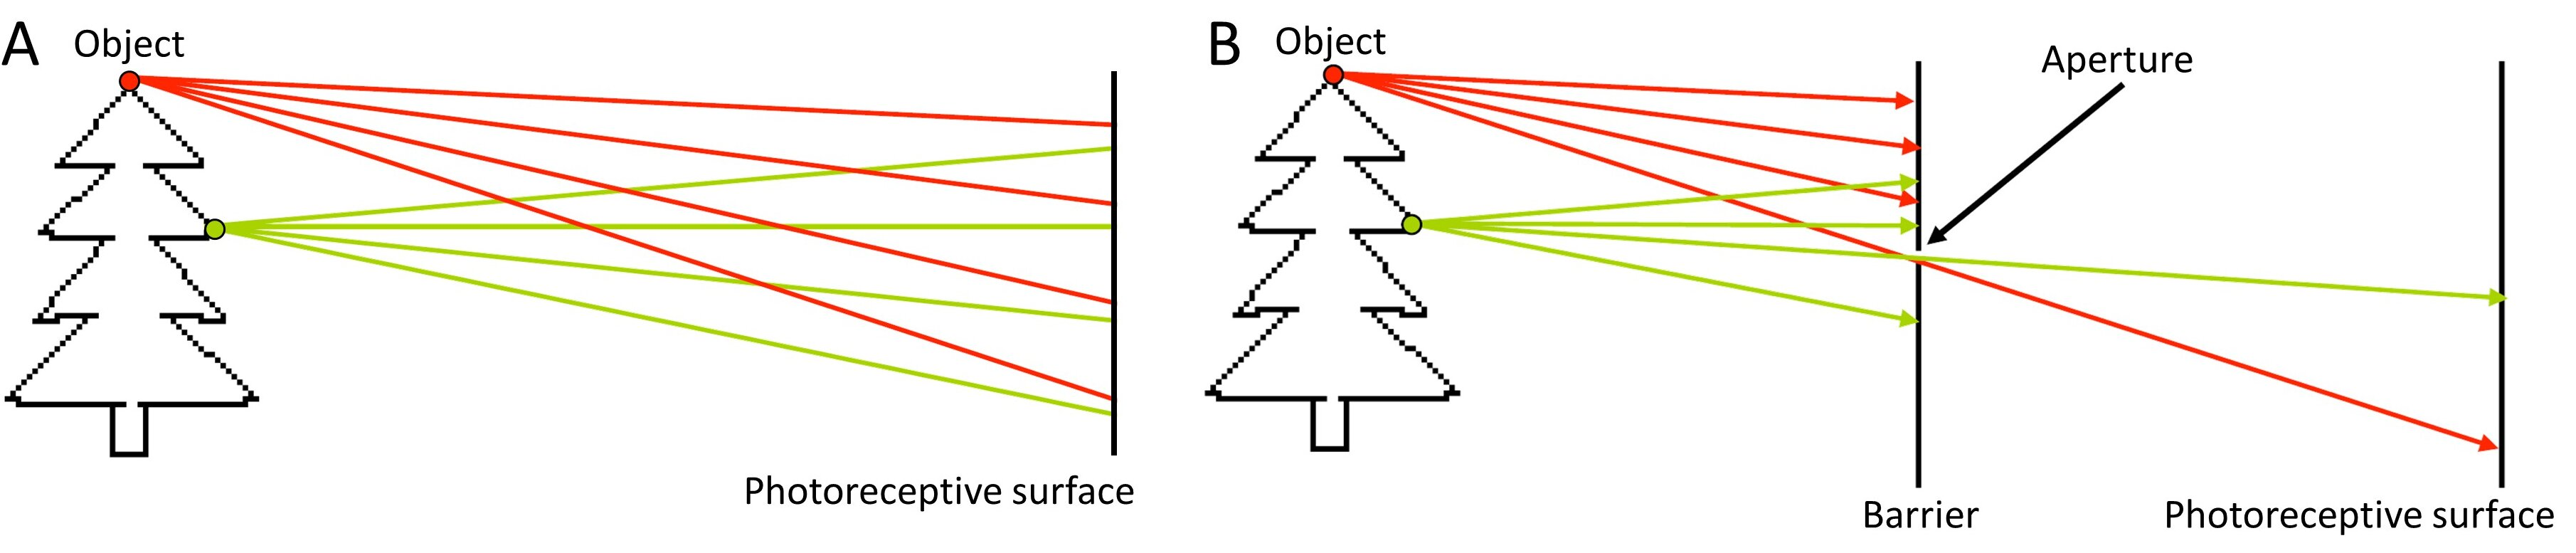
\includegraphics[width=\textwidth]{LightRays0.jpg}
\caption{Light rays on a photoreceptive surface referred to as the image plane. In (A), the image is blurry whereas in (B), a barrier has been added so that "red" and "green" scattered light rays can be distinguished  \cite{FP}.}
\label{fig:LightRays}
\end{figure}

With this basic model for a camera, the geometry can be described with mathematical equations. First, from viewing Figure \ref{fig:PinholeMath}A, one can see that the object as recorded on the image plane is inverted, so often for mathematical derivations, the virtual image plane is used instead. Next, if we define an origin at the pinhole, $o$, in Figure \ref{fig:PinholeMath}B, we can say that point $P$ on the object has coordinates $(-X,Y,-Z)$, while the point $p$ on the image plane has coordinates $(x,-y,f)$ where $f$ is the focal length. By drawing similar triangles, as the points $P$, $o$, and $p$ are collinear, we can write the following equations where the negative signs cancel when using the virtual image plane:

$$\frac{x}{f}=\frac{X}{Z} \ \ ; \ \  \frac{y}{f}=\frac{Y}{Z}$$

We can then solve for $x$ and $y$ which lie on the image plane and are proportional to pixels coordinates which we will later discuss:

$$x=f\frac{X}{Z} \ \ ; \ \ y=f\frac{Y}{Z}$$

\begin{figure} 
\centering
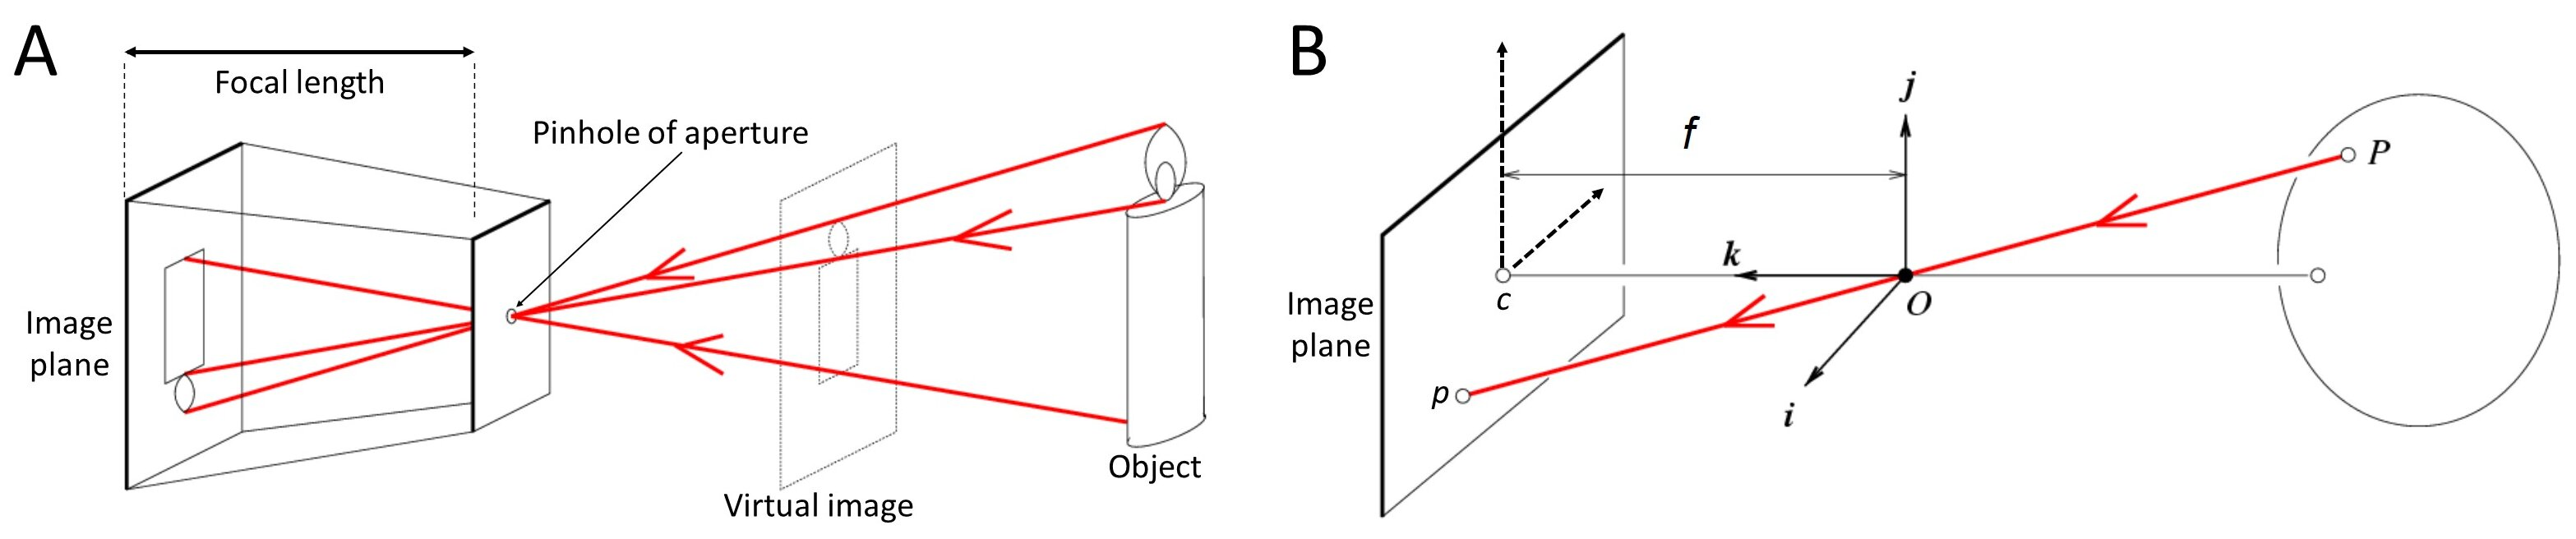
\includegraphics[width=\textwidth]{PinholeMath0.jpg}
\caption{Pinhole camera model. In (A), it can be seen that due to the geometry of the pinhole camera system, the object image is inverted on the image plane and thus, for ease of math, the virtual image plane which displays the non-inverted object is used. In (B), the image center is labeled as $c$, the pinhole is labeled as $o$, the optical axis lies along vector $k$, the focal length is $f$, the 3D point is labeled as $P$, and the 2D pixel point is labeled $p$  \cite{HZ}.}
\label{fig:PinholeMath}
\end{figure}

\subsubsection{Camera lenses}

One limitation of the current pinhole camera model is light. We have already discussed how lacking an aperture, i.e. having an aperture of infinite diameter, leads to a blurry image. But thus far in mathematical terms, we have technically been discussing an aperture of zero diameter which would in reality let in no light. In the middle ground between these two extremes, there is a tradeoff between amount of light that is absorbed by the photoreceptive surface and image blur. Additionally, for small aperture sizes, the resolution becomes fundamentally limited by diffraction in what is called a diffraction-limited system. One clever solution to the lighting-blur issue is to add a lens to replace the aperture as seen in Figure \ref{fig:Lens}A. A lens is an optical element that focuses light by means of refraction. As can be seen however, the light from the object is only focused correctly if the distance to the object equals the focal length of the lens. For any other distance, the image will again appear blurred, although the closer to the focal length distance, the less blur. The size of the 3D region where the blur is acceptably low is called the depth of field.

With this lens, we can now extend our pinhole mathematical model. When looking at Figure \ref{fig:Lens}B, we can use Snell's law and the assumption of a thin lens relative to the focal distance to develop similar triangles. First, rays that pass through the center of the lens are not refracted. Second, rays parallel to the optical axis are focused on the focal point labeled $F'$. Third, all rays passing through point $P$ are focused by the thin lens on the point $p$. Thus, using similar triangles we can write the following equations first using the blue similar triangles then the red similar triangles:

$$\frac{y}{Y}=\frac{z}{Z}=\frac{z-f}{f}$$

Combining these two equations we can write the thin lens equation:

$$\frac{1}{z}+\frac{1}{Z}=\frac{1}{f}$$

We can additionally notice from this geometry that the variable $z$ in the lens model is equivalent to $f$ in the pinhole model and once again notice that points that are not a distance of $Z$ away from the lens will be out of focus. We also see that if $Z$ approaches infinity, light would focus a distance of $f$ away from the lens. Thus, we could assume a pinhole model if the lens is focused at infinity and this could allow us to map 3D points into the camera image plane where they could be converted into pixel coordinates.

\begin{figure} 
\centering
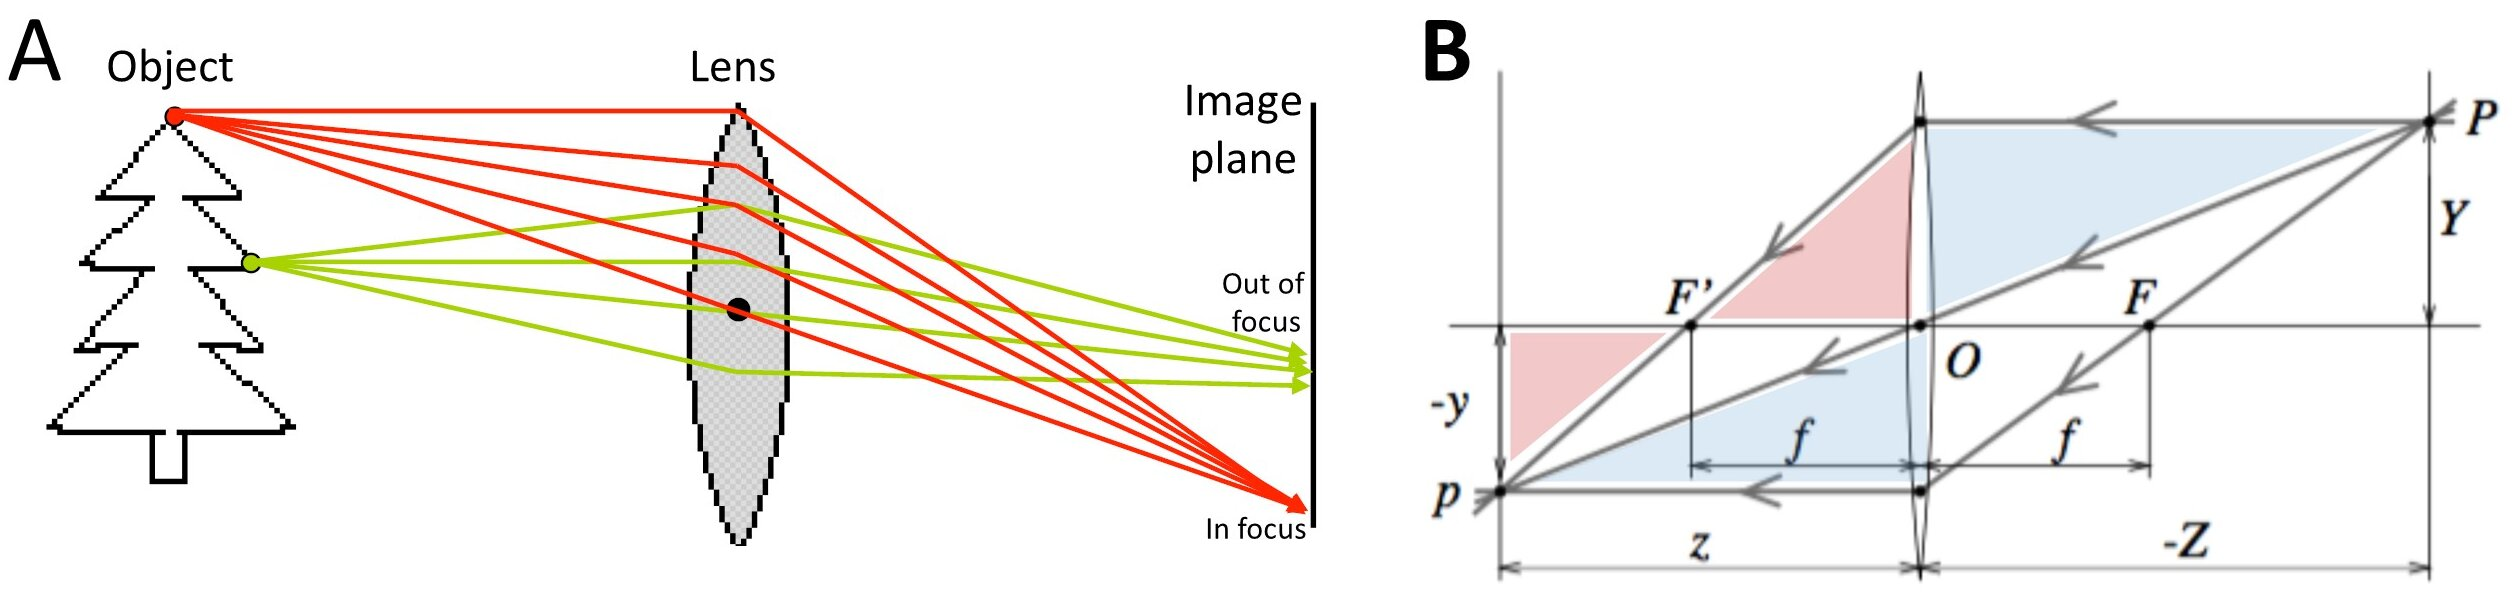
\includegraphics[width=\textwidth]{Lens0.jpg}
\caption{A lens is used to focus light. In (A), a lens is used to focus light originating from an object at a certain distance whereas different distances are blurred. In (B), the thin lens model can be developed using similar triangles  \cite{HZ}.}
\label{fig:Lens}
\end{figure}

\subsubsection{Tradeoffs to optimize light and blur}

With this more complete camera model, we can discuss the tradeoffs involved in most camera applications, especially those involving quickly moving objects, i.e. high-speed cameras. Assuming we want a crisp image without blur, the following factors are critical: object movement, exposure time, receptivity of the photoreceptive surface, aperture size, and lighting conditions. For high speed applications, the exposure time of the camera, or amount of time that the photoreceptive imaging surface absorbs light, needs to be short so that the quickly moving object of interest doesn't move significantly during the exposure time. But with a lower exposure time, less light is absorbed. So to provide more light, we could open the aperture to a larger diameter, but doing so will decrease the depth of field. One solution is to increase the brightness of the light source or sources which is often why extremely bright light sources are used for high speed applications. Regardless, this fundamental issue of light capture exists for cameras especially high-speed cameras, and a proper balance of aperture size and exposure time is needed to optimize blur and image brightness. This, combined with a highly receptive photoreceptive surface and bright lighting conditions need to be considered carefully in photography.

\bibliographystyle{unsrt}%Used BibTeX style is unsrt
\bibliography{reference}
\end{document}